\documentclass[twoside,11pt]{article}

% Any additional packages needed should be included after jmlr2e.
% Note that jmlr2e.sty includes epsfig, amssymb, natbib and graphicx,
% and defines many common macros, such as 'proof' and 'example'.
%
% It also sets the bibliographystyle to plainnat; for more information on
% natbib citation styles, see the natbib documentation, a copy of which
% is archived at http://www.jmlr.org/format/natbib.pdf

\usepackage{jmlr2e}

\usepackage{booktabs}
%\usepackage{graphicx}
\usepackage[tableposition=top]{caption}
\usepackage{lipsum}
\usepackage{diagbox}
\usepackage{rotating}
\usepackage{subcaption}
\usepackage{multirow}

% Definitions of handy macros can go here

\newcommand{\dataset}{{\cal D}}
\newcommand{\fracpartial}[2]{\frac{\partial #1}{\partial  #2}}

% Heading arguments are {volume}{year}{pages}{date submitted}{date published}{paper id}{author-full-names}

% \jmlrheading{1}{2000}{1-48}{4/00}{10/00}{meila00a}{Marina Meil\u{a} and Michael I. Jordan}

% Short headings should be running head and authors last names

\ShortHeadings{Performance of Six Algorithms on Five Binary Classification Problems}{Siemers}
\firstpageno{1}

\begin{document}
	
	\title{Empirical Study of the Performance of Six Algorithms on Five Binary Classification Problems}
	
	\author{\name Maximilian Siemers \email siemersm@gmail.com \\
		\addr Department of Cognitive Science\\
		University of California, San Diego\\
		San Diego, CA 92117, USA}
	
	\course{COGS 118A: Introduction to Machine Learning I}
	\prof{Prof. Zhuowen Tu}
	
	\maketitle
	
	\begin{abstract}%   <- trailing '%' for backward compatibility of .sty file
		
	\end{abstract}
	
	\begin{keywords}
		
	\end{keywords}

	
	\section{Introduction}
	
	\section{Method}
		% - Data desc
		% - CLF desc
		% - Hyperparam desc
		
		\subsection{Problems}
			% Data size table
			\begin{table}[h]
				\captionbox{Original and limited sizes of data sets}{
				\label{tab:data_sizes}
				\begin{tabular}{lll}
					\toprule
					Data set & Orig. Size & Lim. Size \\
					\midrule
					COVTYPE	& $(581011 \times 55)$	& $(2000 \times 55) $ \\
					INCOME	& $(32561 \times 109)$	& $(2000 \times 109) $ \\
					LETTER	& $(20000 \times 16)$	& ($2000 \times 16) $ \\
					IRIS	& \multicolumn{2}{c}{--- $(150 \times 5)$ ---} \\
					WDBC	& \multicolumn{2}{c}{--- $(569 \times 31)$ ---} \\
					\bottomrule
				\end{tabular}}
			\end{table}
	
	\section{Experiments}
		
		\subsection{Hyperparameters and Performance}
			% Hyperparam figures # 1
			\begin{figure}[h]
				\centering
				
				\begin{subfigure}[b]{.45\linewidth}
					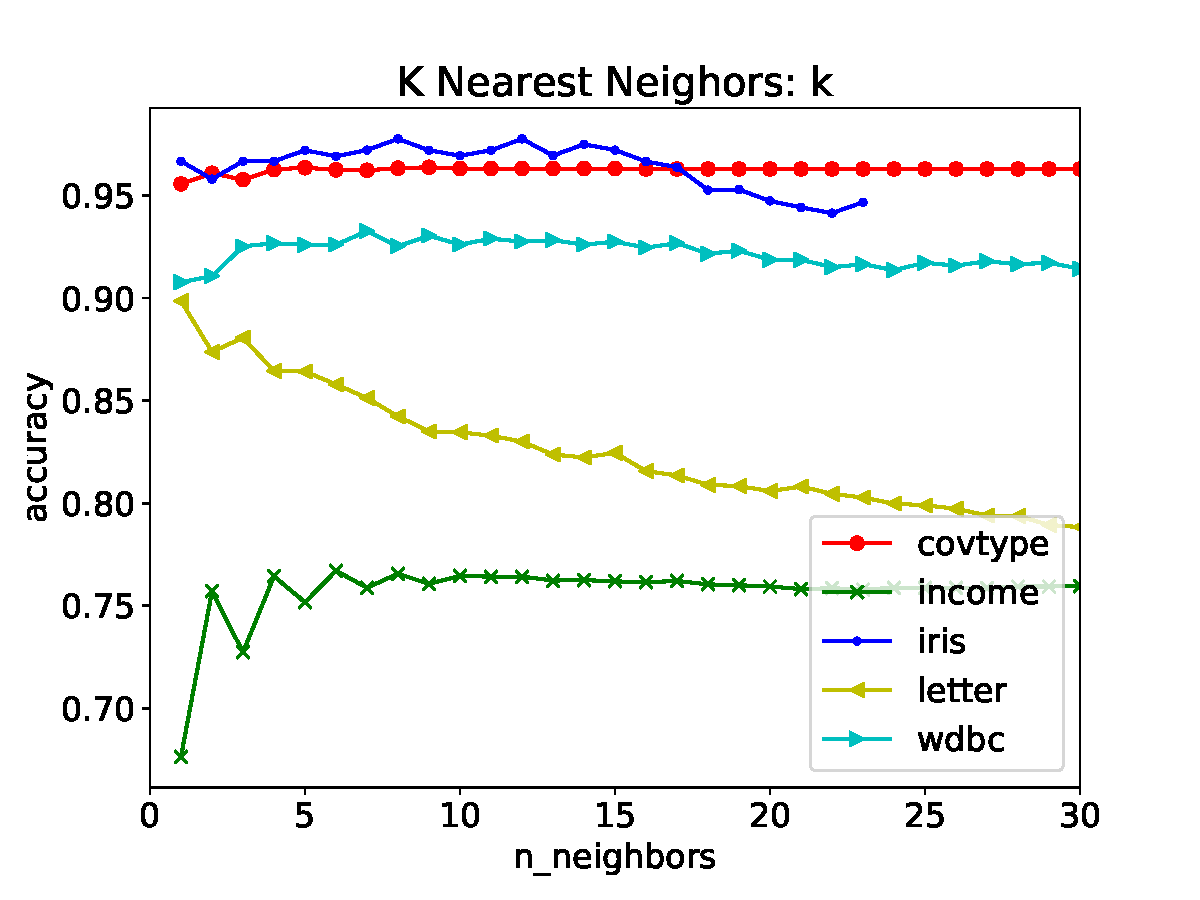
\includegraphics[width=\linewidth]{knn_hyperparam_zoomed}
					\caption{KNN: \textit{k}}
					\label{fig:hyperparam_knn_zoomed}
				\end{subfigure}
				\begin{subfigure}[b]{.45\linewidth}
					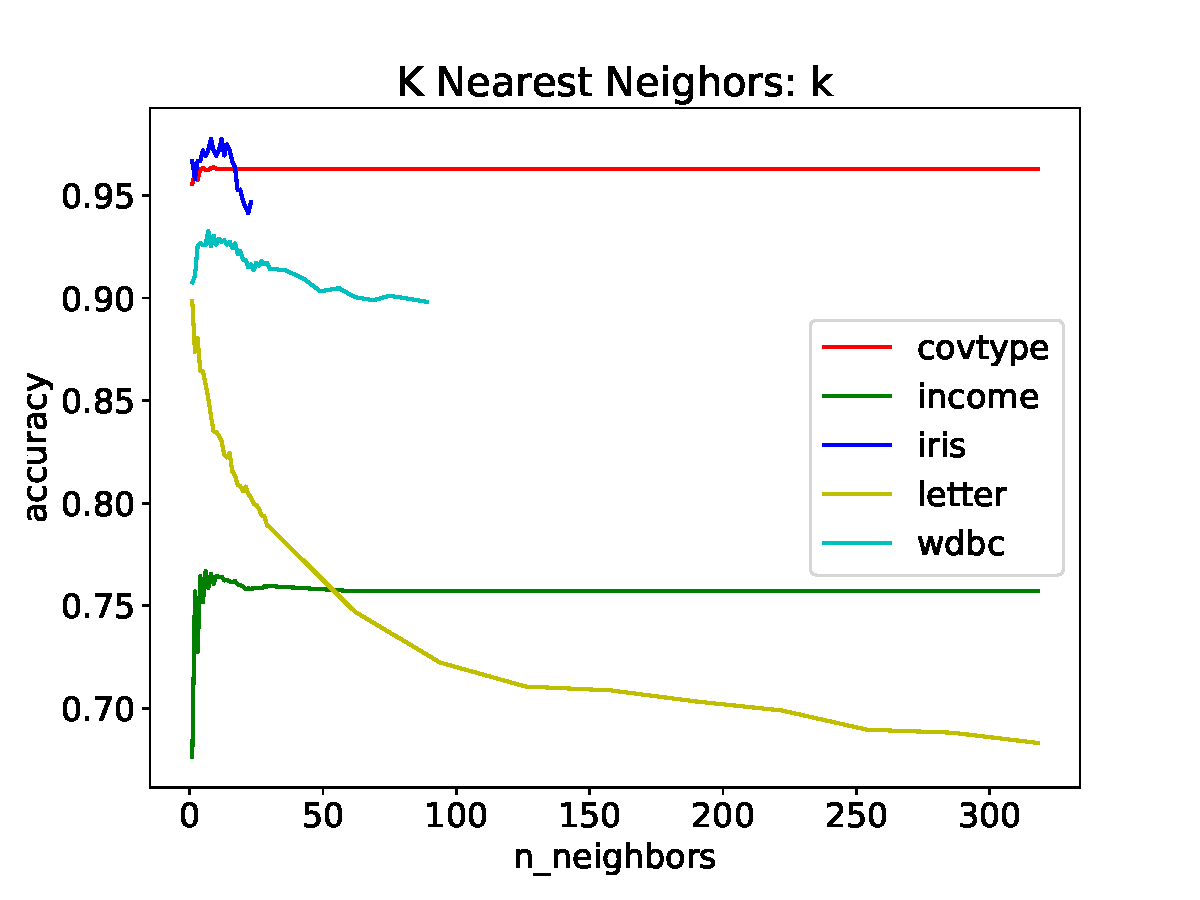
\includegraphics[width=\linewidth]{knn_hyperparam_all}
					\caption{KNN: \textit{k}}
					\label{fig:hyperparam_knn_all}
				\end{subfigure}
			
				\begin{subfigure}[b]{.45\linewidth}
					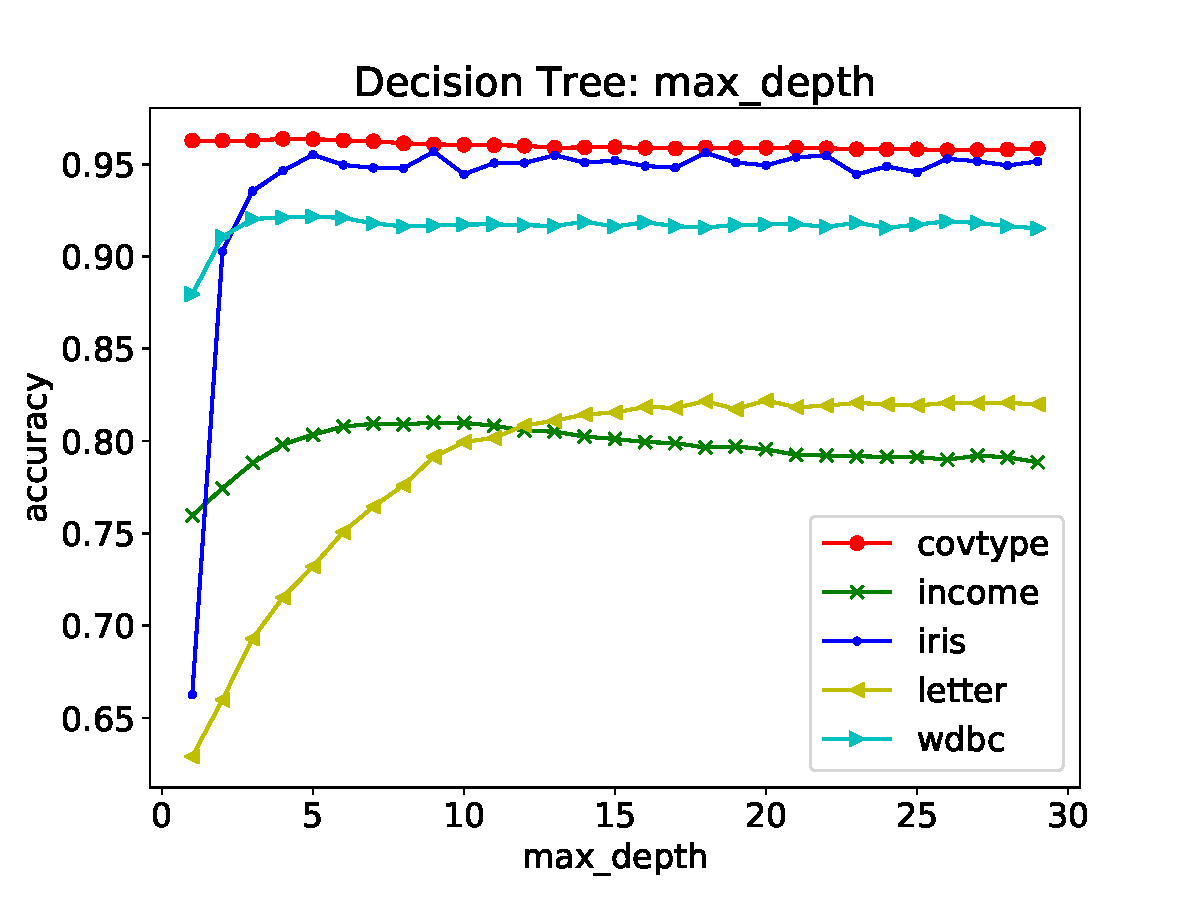
\includegraphics[width=\linewidth]{dt_hyperparam_max_depth}
					\caption{Decision Tree: \textit{max\_depth}}
					\label{fig:hyperparam_dt_max_depth}
				\end{subfigure}
				\begin{subfigure}[b]{.45\linewidth}
					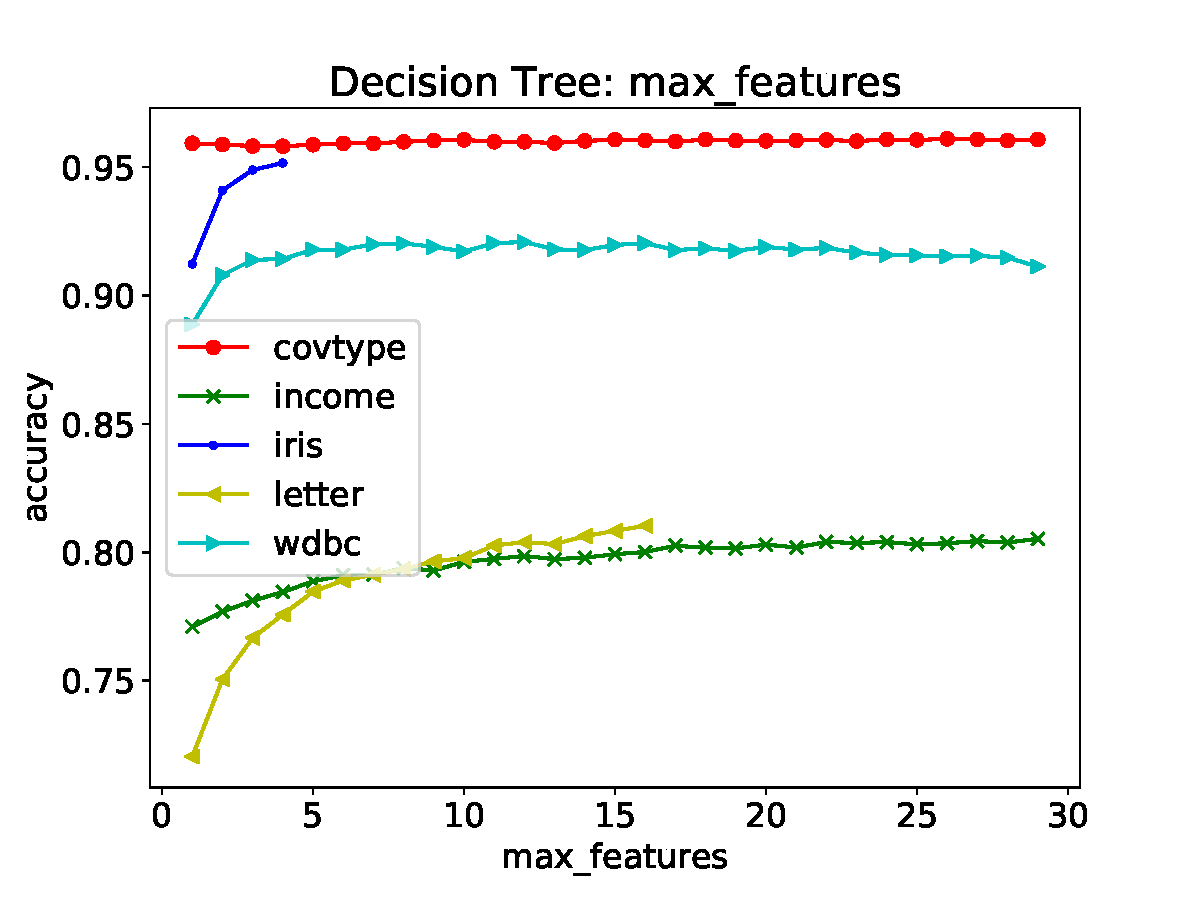
\includegraphics[width=\linewidth]{dt_hyperparam_max_features}
					\caption{Decision Tree: \textit{max\_features}}
					\label{fig:hyperparam_dt_max_features}
				\end{subfigure}
				
				\caption{Validation score by hyperparameter value for KNN (\ref{fig:hyperparam_knn_zoomed} and \ref{fig:hyperparam_knn_all}) and Decision Tree (\ref{fig:hyperparam_dt_max_depth} and \ref{fig:hyperparam_dt_max_features}), averaged over data, shuffles, and train split. \ref{fig:hyperparam_knn_zoomed} zooms in on a subset of the results shown in \ref{fig:hyperparam_dt_max_depth} for greater detail. \ref{fig:hyperparam_dt_max_depth} depicts results for varying levels of \textit{max\_depth}, averaged over \textit{max\_features}, wheres the opposite is done in \ref{fig:hyperparam_dt_max_depth}.}
				\label{fig:hyperparam_knn_dt}
			\end{figure}
			
			% Hyperparam figures # 2
			\begin{figure}[h]
				\centering
				
				\begin{subfigure}[b]{.45\linewidth}
					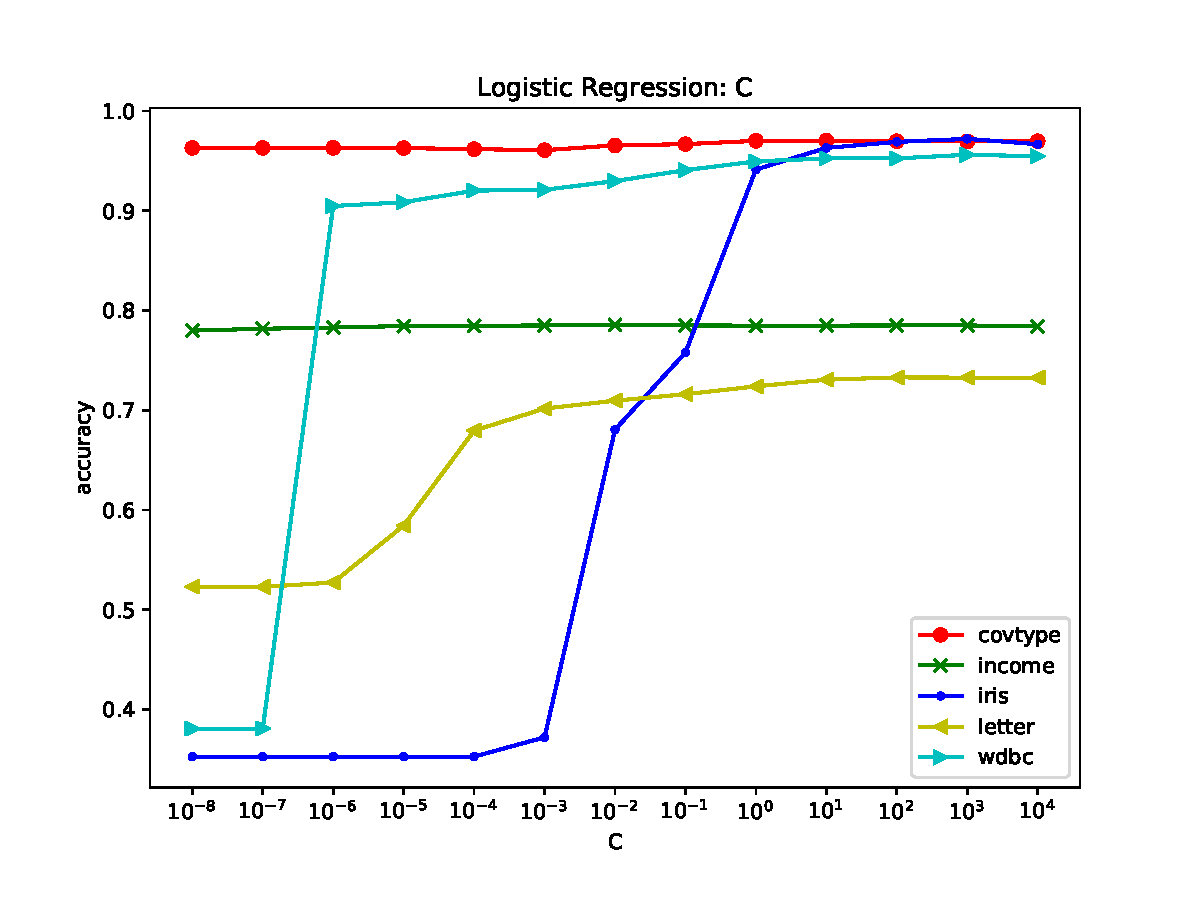
\includegraphics[width=\linewidth]{logreg_hyperparam}
					\caption{Logistic Regression: \textit{C}}
					\label{fig:hyperparam_logreg}
				\end{subfigure}
				\begin{subfigure}[b]{.45\linewidth}
					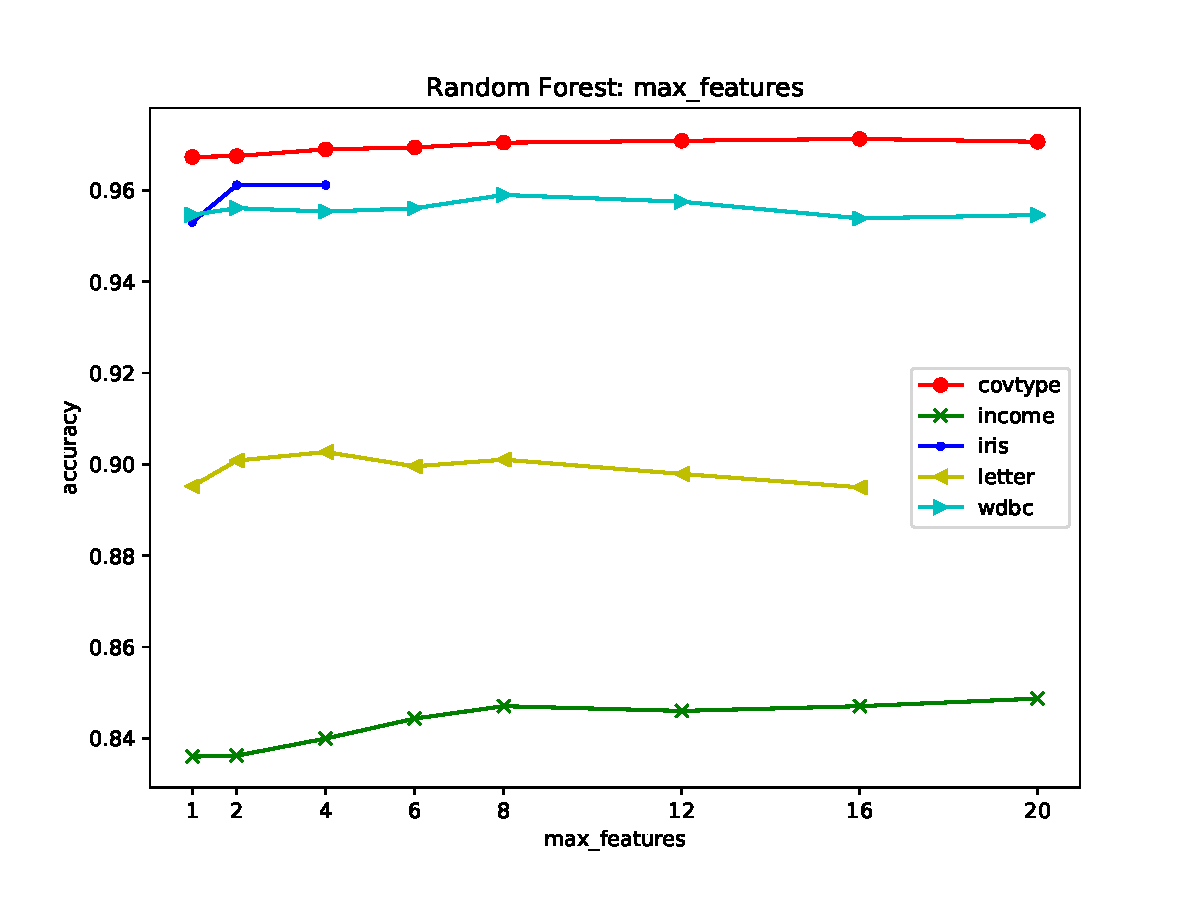
\includegraphics[width=\linewidth]{rf_hyperparam}
					\caption{Random Forest: \textit{n\_estimators}}
					\label{fig:hyperparam_rf}
				\end{subfigure}
				
				\begin{subfigure}[b]{.45\linewidth}
					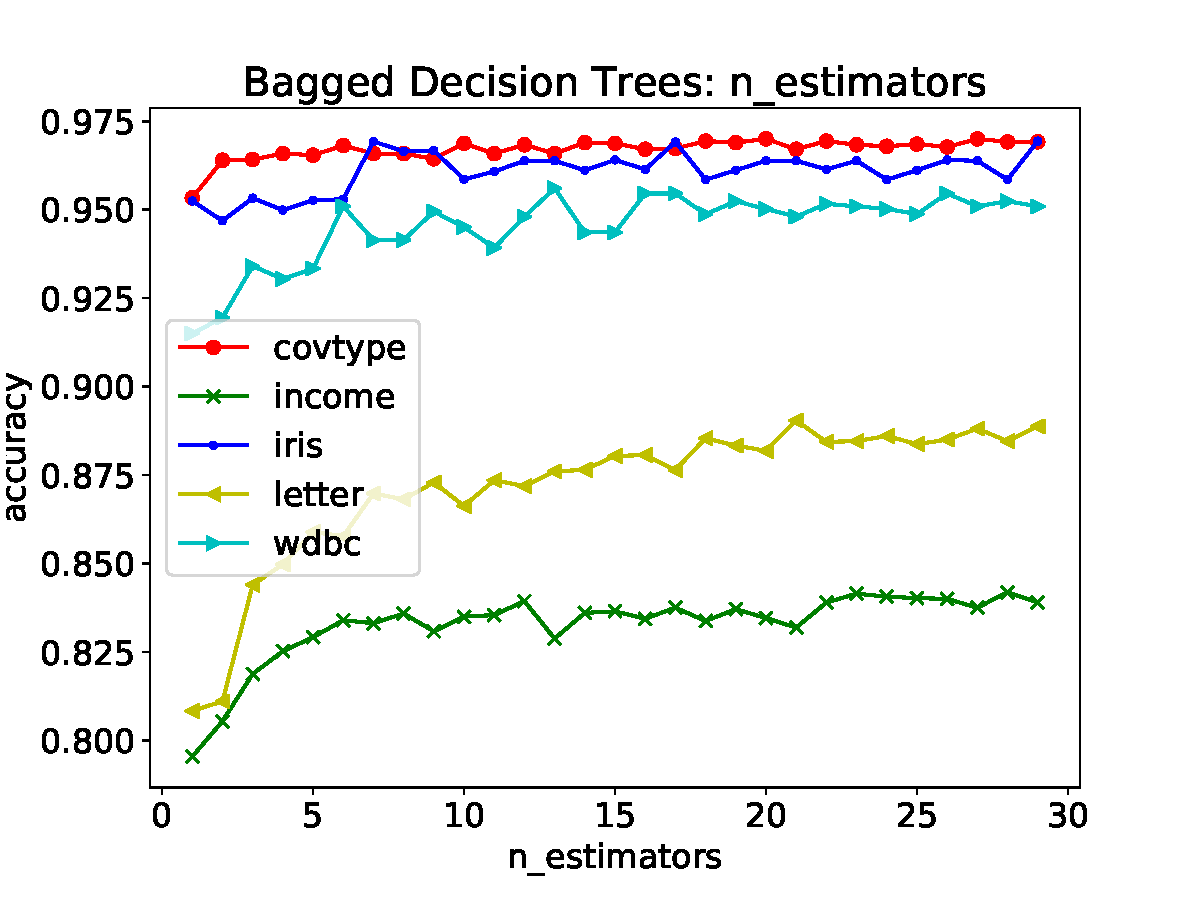
\includegraphics[width=\linewidth]{bagdt_hyperparam}
					\caption{Bagged Decision Trees: \textit{n\_estimators}}
					\label{fig:hyperparam_bagdt}
				\end{subfigure}
				\begin{subfigure}[b]{.45\linewidth}
					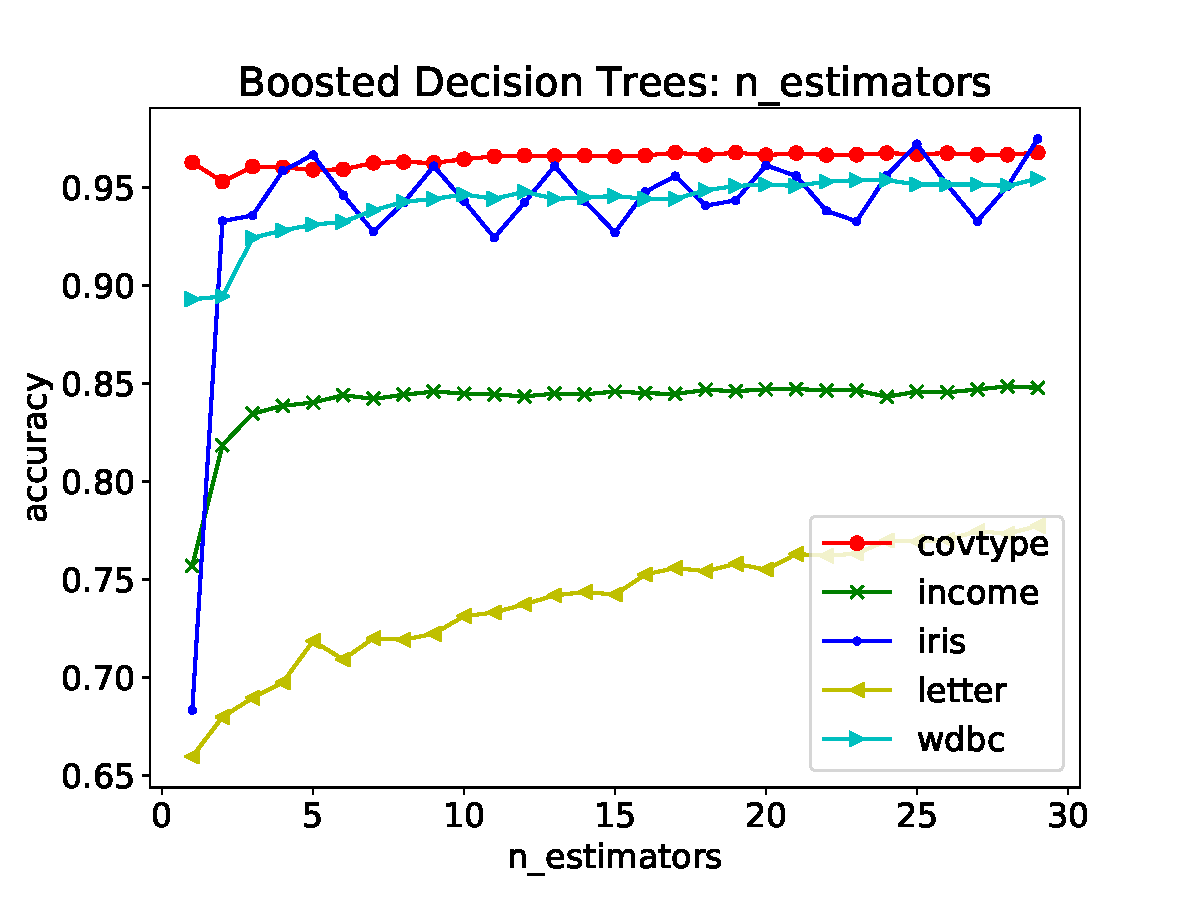
\includegraphics[width=\linewidth]{bstdt_hyperparam}
					\caption{Boosted Decision Trees: \textit{n\_estimators}}
					\label{fig:hyperparam_bstdt}
				\end{subfigure}
				
				\caption{Validation score by hyperparameter value for Logistic Regression (\ref{fig:hyperparam_logreg}), Random Forest (\ref{fig:hyperparam_rf}), Bagged Decision Trees (\ref{fig:hyperparam_bagdt}), and Boosted Decision Trees (\ref{fig:hyperparam_bstdt}).}
				\label{fig:hyperparam_others}
			\end{figure}
		
		\subsection{Train/Test split and Performance}
			\begin{figure}[h]
				\begin{subfigure}{.5\textwidth}
					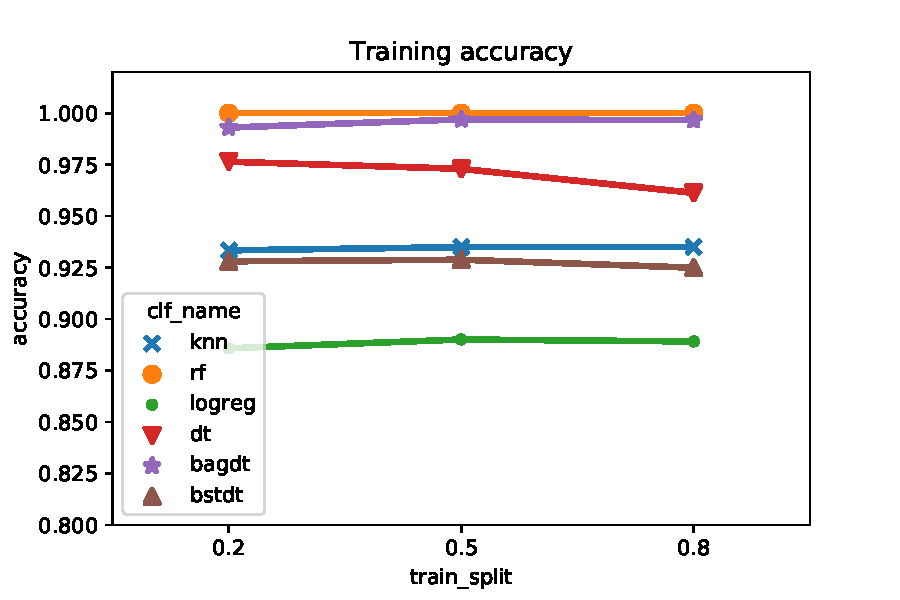
\includegraphics[width=\textwidth]{tr_acc_by_clf_trainsplit}
					\caption{Training accuracy}
					\label{fig:perf_by_trainsplit_tr}
				\end{subfigure}
				\begin{subfigure}{.5\textwidth}
					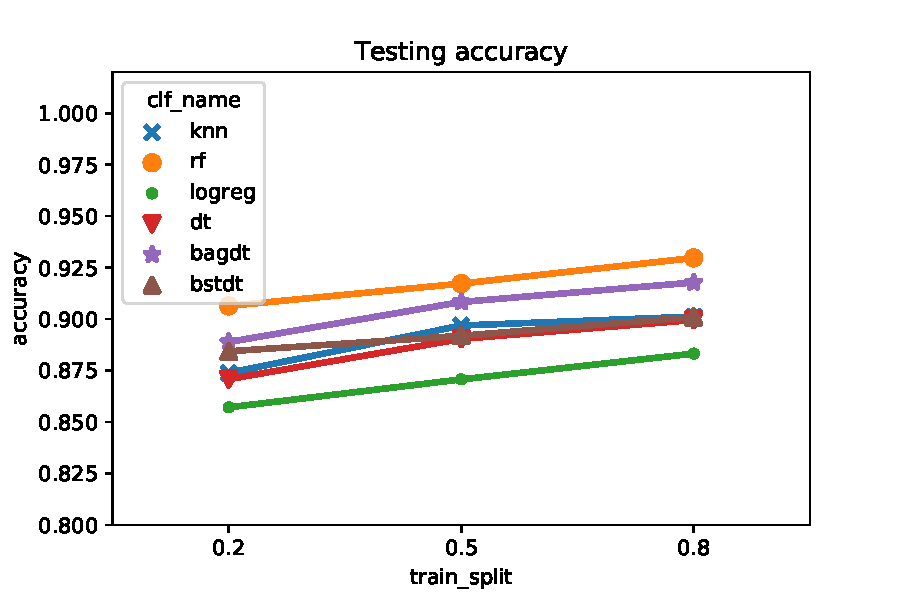
\includegraphics[width=\textwidth]{te_acc_by_clf_trainsplit}
					\caption{Testing accuracy}
					\label{fig:perf_by_trainsplit_te}
				\end{subfigure}
				\caption{Training (\ref{fig:perf_by_trainsplit_tr}) and testing (\ref{fig:perf_by_trainsplit_te}) accuracy by train split and classifier, averaged over problems and shuffles (rf: Random Forest, logreg: Logistic Regression, dt: Decision Tree, bagdt: Bagged Trees, bstdt: Boosted Trees)}
				\label{fig:perf_by_trainsplit}
			\end{figure}
		
		\subsection{Overall Classifier Performance}
			
			% Model selection results: Best hyperparams
			\begin{table}[ph!]
				\caption{Best hyperparameter values after grid search by classifier and problem in each of three random shuffles (0.8 train split):}
				\label{tab:best_hyperparams_by_problem_shuffles}
				\begin{tabular}{lllllll}
					\toprule
					& & \multicolumn{5}{c}{Problem} \\\cline{3-7}
					Classifier & Hyperparam. &         COVTYPE &           INCOME &               IRIS &              LETTER &                 WDBC \\
					\midrule
					bagdt & \textit{n\_estimators} &         3,27,14 &         26,25,28 &             9,29,7 &            21,14,18 &              13,9,16 \\
					bstdt & \textit{n\_estimators}  &        24,19,12 &         28,18,18 &            5,29,24 &            29,28,24 &             21,29,10 \\
					\multirow{2}{*}{dt} & \textit{max\_depth} &           3,5,4 &            8,4,6 &              9,9,3 &            18,19,18 &                6,5,6 \\
					& \textit{max\_features} &        18,24,19 &         18,24,26 &              3,4,4 &             10,15,6 &              7,11,15 \\
					knn & \textit{n\_neighbors} &           4,5,9 &           8,6,17 &             12,9,1 &               1,1,1 &                9,7,7 \\
					logreg & \textit{C} &  $10^2$,1,10 &  1e-05,01,01 &  10,$10^3$,$10^2$ &  $10^2$,$10^3$,$10^2$ &  $10^3$0,10,$10^3$ \\
					\multirow{2}{*}{rf} & \textit{max\_features} &        20,16,16 &          20,16,8 &              1,2,2 &               4,2,8 &               12,8,8 \\
					& \textit{n\_estimators} &  $2^{10}$,$2^{10}$,$2^{10}$ &   $2^{10}$,$2^{10}$,$2^{10}$ &     $2^{10}$,$2^{10}$,$2^{10}$ &      $2^{10}$,$2^{10}$,$2^{10}$ &       $2^{10}$,$2^{10}$,$2^{10}$ \\
					\bottomrule
				\end{tabular}
			
			\end{table}
			
			% Overall average results of clfs on datasets
			\begin{table}[h]
				\captionbox{Classifier testing accuracy by problem, averaged over shuffles (0.8 train split):}{
				\begin{tabular}{lrrrrr}
					\toprule
					Classifier & WDBC & INCOME & IRIS & COVTYPE & LETTER \\
					\midrule
					Bagged Trees  & .968 &   .833 & .944 &    .971 &   .873 \\
					Boosted Trees  & .968 &   .840 & .956 &    .971 &   .771 \\
					Decision Tree     & .953 &   .799 & .956 &    .970 &   .820 \\
					KNN    & .950 &   .757 & .933 &    .967 &   \textbf{.899} \\
					Logistic Regression & .968 &   .792 & \textbf{.967} &    .968 &   .721 \\
					Random Forest     & \textbf{.982} &   \textbf{.848} & .944 &    \textbf{.976} &   .897 \\
					\bottomrule
				\end{tabular}}
			\end{table}
		
			% Overall average results of clfs, sorted
			\begin{table}[h]
				\captionbox{Ranked classifiers by testing accuracy, averaged over problems and shuffles (0.8 train split):}{
				\label{tab:clf_ranking}
				\begin{tabular}{lr}
					\toprule
					{Classifier} & Accuracy \\
					\midrule
					Random Forest     &     .930 \\
					Bagged Trees  &     .918 \\
					KNN    &     .901 \\
					Boosted Trees  &     .901 \\
					Decision Tree     &     .900 \\
					Logistic Regression &     .883 \\
					\bottomrule
				\end{tabular}}
			\end{table}
	
	\section{Conclusion}
	
	\section{Bonus Points}
	
	\section{References}
	
	
	
	
	
	
	
	\newpage
	
	\appendix
	\section*{Appendix A.}
	\label{app:theorem}
	
	
	
	\vskip 0.2in
	\bibliography{sample}
	
\end{document}